\part{Conclusion et perspective}
\section{Recette}
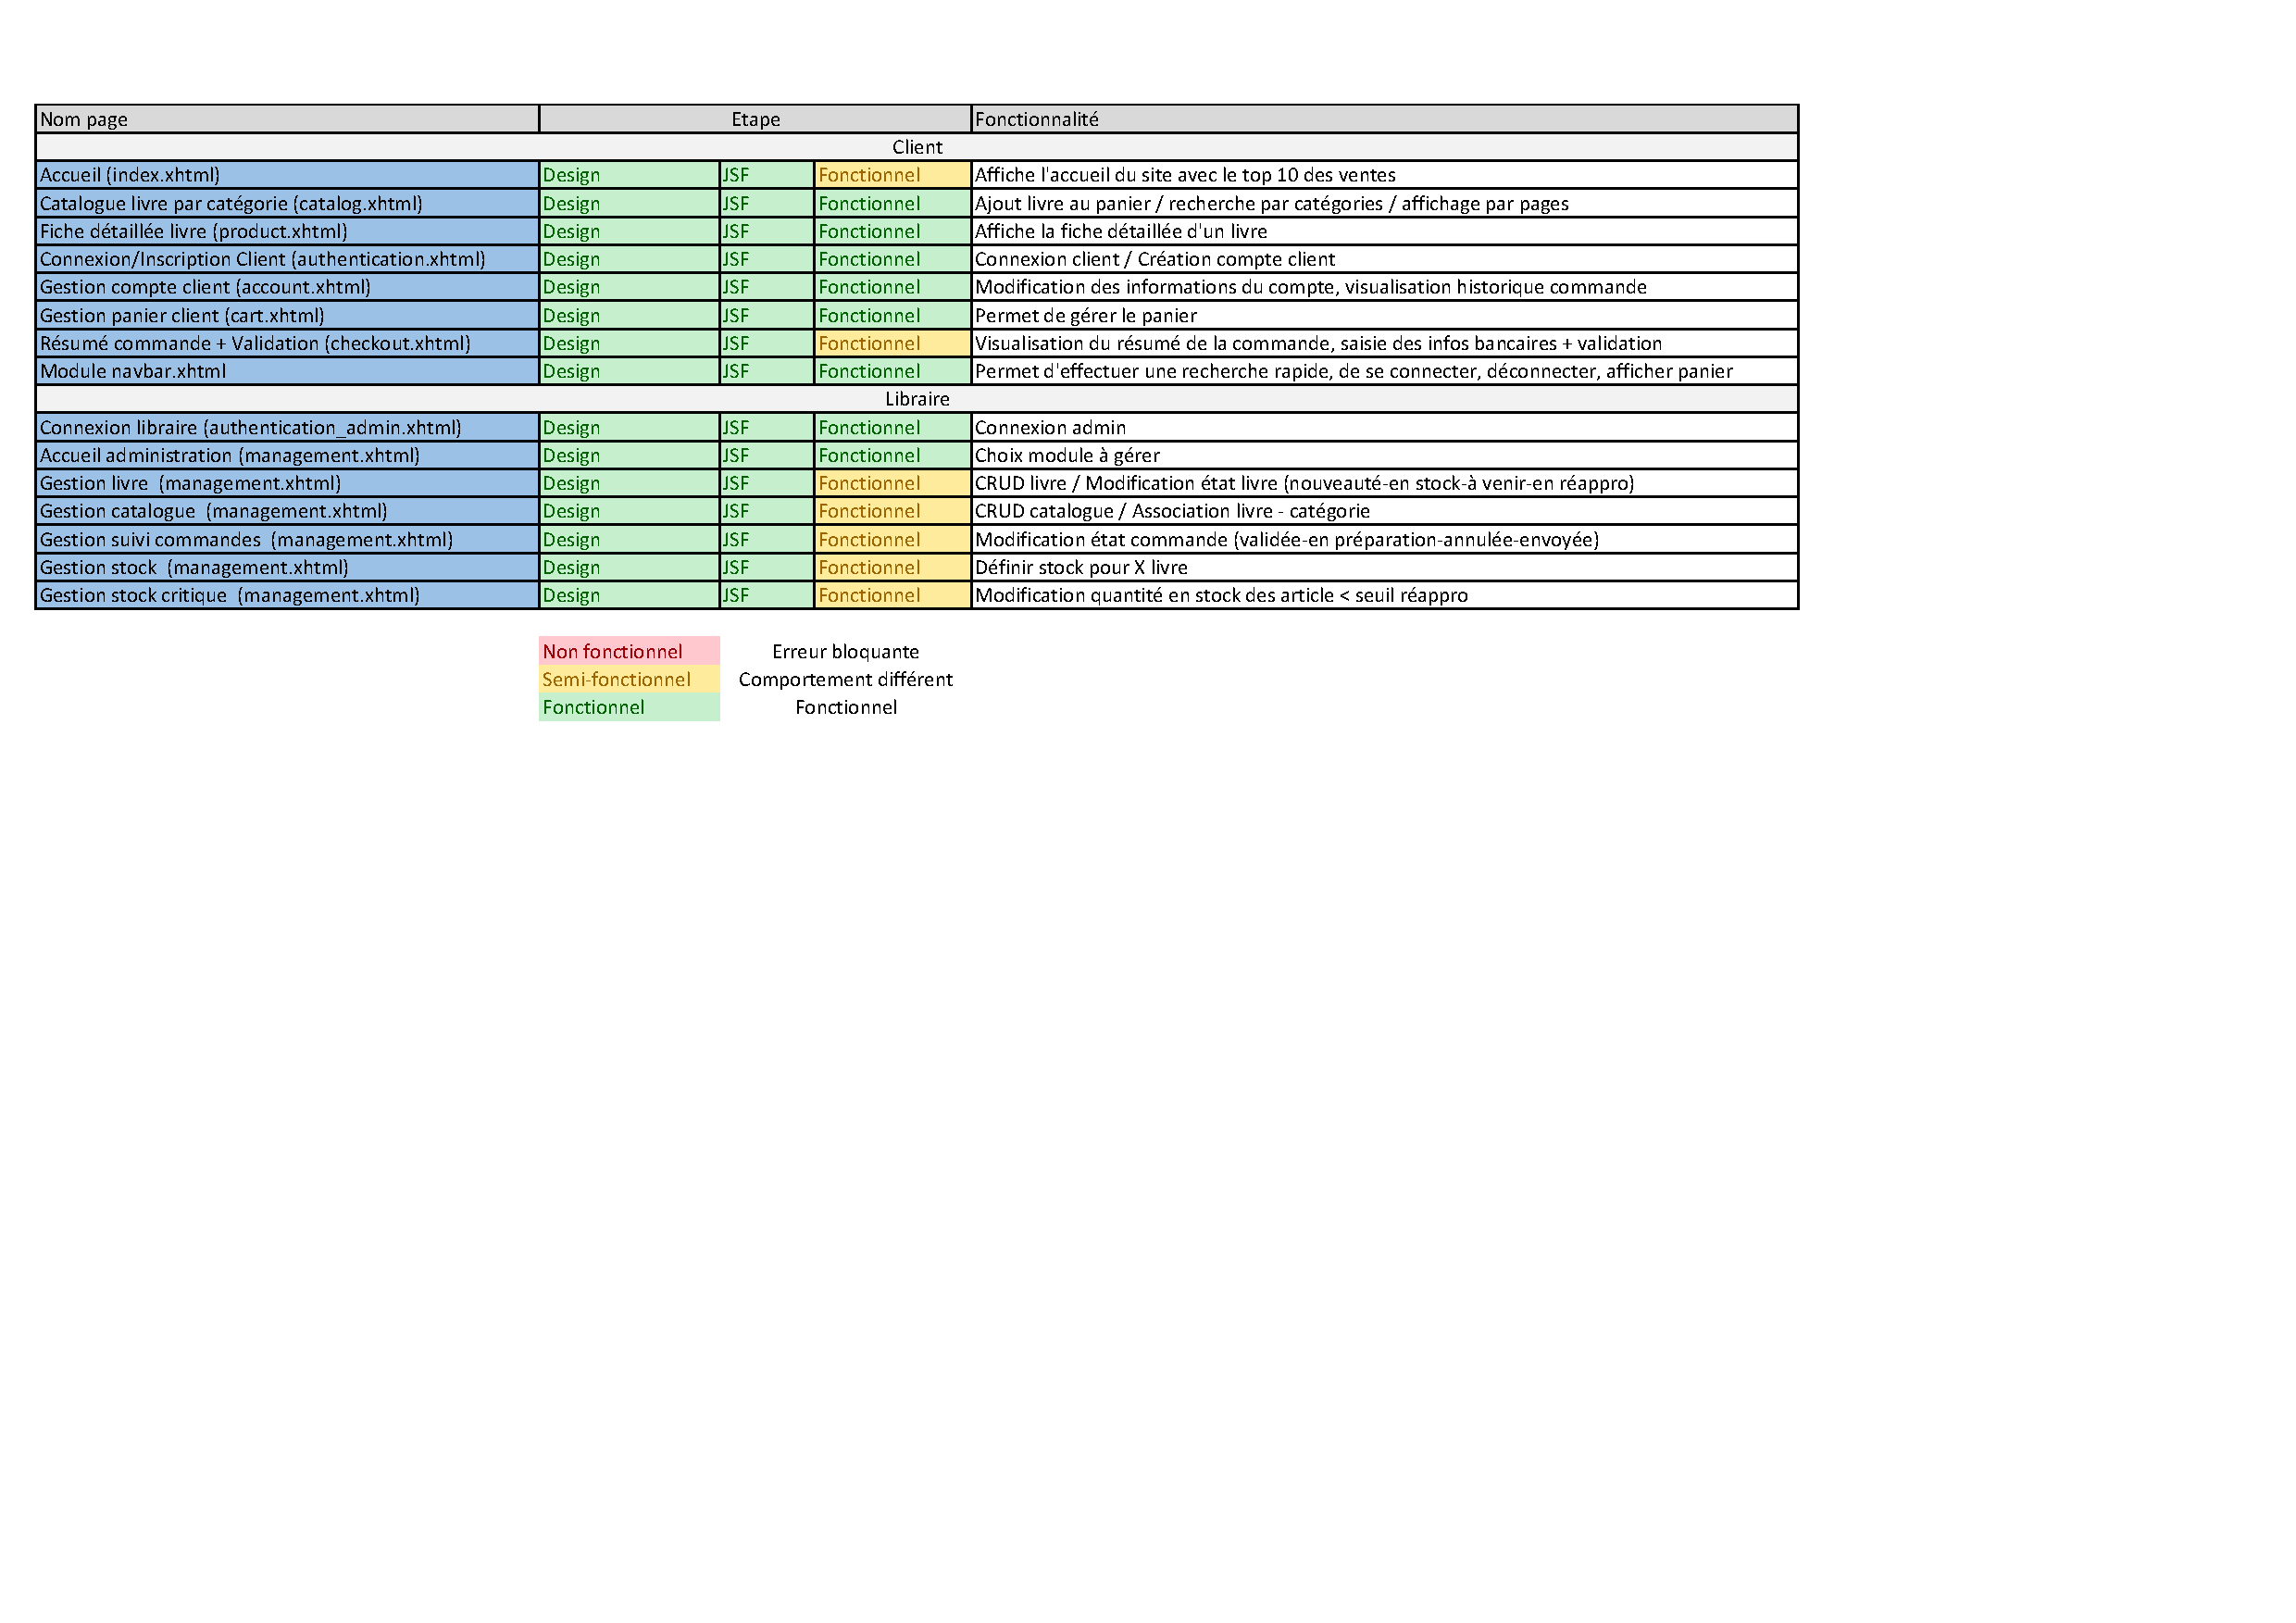
\includepdf[scale=1.2,landscape=true,offset=150 100]{Res/listing_page.pdf}
\section{Analyse des écarts}
\section{Évolutions proposées}

	\subsection{Dynamiser la recherche}

	La recherche est actuellement tout ce qu'il y a de plus statique. Simple, classique, efficace. Mais il est possible d'améliorer et de fluidifier l'expérience utilisateur.

	\begin{itemize}
		\item Utiliser des suggestions de recherches. Comme son nom l'indique, cela consiste à suggérer des résultats à l'utilisateur, lorsqu'il tape sa recherche. Un tel système, bien implémenté, permet à l'utilisateur de trouver avant même d'avoir fini de taper.
		\item Recharger dynamiquement la page. Actuellement, la page est rechargée dans son intégralité lorsqu'une recherche est effectuée. Il est possible de ne recharger qu'une partie de la page (ici, la partie affichant les résultats de recherche), pour au final une expérience plus fluide.
	\end{itemize}

	\subsection{Tenir l'utilisateur informé}

	Il pourrait être possible de tenir l'utilisateur informé des événements importants de notre librairie. On peut imaginer un système d'abonnement via newsletter ou flux RSS. Un abonnement aux dernières sorties d'un genre ou d'un auteur particulier permettrait de tenir le lecteur informé des sujets qui l'intéressent.

	\subsection{Clarifier l'administration}

	L'interface d'administration du libraire doit présenter beaucoup d'informations. Implémenter un système similaire à un tableur, où le libraire est en mesure de choisir quelles informations afficher, et les trier plus librement serait une amélioration pour la lisibilité.

	\subsection{Dynamiser le suivi des commandes}

	Il serait possible d'intégrer un indicateur à la barre de navigation, qui afficherait en temps réel les informations concernant la dernière commande de l'utilisateur.

\section{Bilans personnels et de groupe}


\subsection{Cyril LE ROY}
Ce projet m’a appris deux choses.
La première, je n’aime pas Java EE. Quand on est habitué à développer des sites Web du même genre que BooXtore de manière simple et rapide, il est difficile de passer à la plateforme Java, à GlassFish et ses maudites erreurs de déploiement qui font perdre énormément de temps, aux chargements interminables et j’en passe.

Cependant, le fait de travailler en architecture MVC et d’être supporté par le langage Java (qui reste un langage très puissant et utile pour un développeur grâce à ses librairies riches) est très intéressant car cela se rapproche de nombreux Frameworks PhP et facilite donc de nombreuses étapes de développement.

Évidemment, il est frustrant de passer beaucoup plus de temps à l’apprentissage et donc au développement sur des fonctionnalités qui semblent simples.

Pour conclure, je dirais que je viens tout juste de me rendre compte que depuis deux ans je me plains du manque de temps sur les projets et de ma frustration éternelle sur le fait de ne jamais pouvoir présenter un résultat digne de ce nom.

\subsection{Antoine-Ali ZARROUK}
Je trouve que Java EE est une technologie intéressante, cependant, je trouve la technologie JSF/JSP assez limitante par rapport à un framework graphique type Vaadin.

Bootstrap à été une bonne surprise de par sa flexibilité et sa facilité d'utilisation.

Cependant, diviser le temps par deux pour un tel projet suppose que tout le groupe soit au top concernant la technologie

\subsection{Benjamin ROBERT}
Acclimatation obligatoire pour un environnement tel que le Java EE, où l'architecture d'une application légère peut prendre des allures d'application lourde seulement avec un langage.

Néanmoins, pas d'insatisfaction à la pensée de réaliser un site d'e-commerce pour la mise en application de ce langage. De bonnes surprises quant aux différents outils utilisés, tels que BootStrap ou Git. Une expérience trop courte par rapport aux cahier des charges qui peut rapidement être conséquent sur les petites fonctionnalités.

\subsection{Julien NORMAND}
Pour ce premier projet à l'EXIA.CESI, ça été une grande découverte. Dans un premier temps, il m'a fallu prendre connaissance du fonctionnement d'un projet, les documents que nous sommes amenés à rendre ou à faire. Et la principale chose, comment était partagé le projet.

Concernant le projet en lui même, il était intéressant car on voyait plus en détails comment fonctionnait le JSF dans du Java EE. Vu mon niveau moyen en JAVA, je ne pensais pas parvenir à comprendre ce que je devais faire concernant ma partie.

\subsection{Jordan NOURRY}
Dans les grandes lignes :
	\begin{itemize}
		\item Je trouve Java EE encore plus désagréable à utiliser que Java SE.
		\item Bootstrap est vraiment un beau framework. Le prototypage y est très rapide, et il est simple de récupérer les sources pour les recompiler et avoir des CSS qui possèdent une vraie personnalité - tout en se basant sur une architecture très solide.
		\item C'est le première fois que j'utilise un logiciel de gestion de versions en conditions réelles. Ça aide énormément, d'autant plus lors du travail en groupe.
	\end{itemize}

\subsection{Bilan de groupe}
Ce projet a été un vrai challenge. Outre le fait de la complexité du projet pour à peine une semaine de développement, la conduite du projet aura été semée d’embûches.

Tout d’abord, nous avons perdu un peu de temps en voulant utiliser un Framework de conception d’interfaces Web pour application Java appelé Vaadin. Au départ, les développeurs semblaient enthousiastes à l’idée d’utiliser ce Framework proposé par l’un des développeurs. Mais au vu de ces différentes utilisations de ce Framework, il semblait évident qu’il n’était pas du tout adapté à la conception de site Web tel que BooXtore. J’ai donc dû prendre la décision de rester sur JSF par sécurité, même si cela nous obligeait à reprendre une partie du travail.

La deuxième embûche est arrivée au milieu du développement. Nos entités avaient été générées grâce à la base de données conçue précédemment mais des erreurs bloquantes insolvables nous empêchaient toute avancée. La décision a donc été prise de laisser tomber la base de données et de recréer nous-mêmes nos entités depuis le début, et ce, deux jours avant la fin de la phase de développement. Cette décision était certes un pari, et un pari gagnant car nous avons vite pu faire de grands progrès. Cependant, le goût amer du temps perdu sur un projet court a été assez démoralisant.

Pour conclure, je ferais part de ma déception envers mon propre travail de chef de projet. J’étais vraiment motivé à conduire ce groupe de projet avec une bonne méthode de développement mais ce n’est que rendu à la fin que je me rends compte d’avoir peut être mal utilisé les ressources du projet et le temps alloué.

